\subsection{等差数列}\label{subsec:2-2}

考察上一节中到过的数列
\begin{gather}
    4,\; 5,\; 6,\; 7,\; 8,\; 9,\; 10 \text{。} \tag{$1$}\label{eq:shulie-1-ref}
\end{gather}

我们可以发现,这个数列有这样的特点:从第 $2$ 项起,每一项与它的前一项的差都等于 $1$ 。

一般地,如果一个数列从第 $2$ 项起, 每一项与它的前一项的差等同一个常数,这个数列就叫做\textbf{等差数列},
这个常数叫做等差数列的\textbf{公差}, 公差通常用字母 $d$ 表示。 例如, 数列
$$ 1,\; 3,\; 5,\; 7,\; \cdots $$
与
$$ 5,\; 0,\; -5,\; -10,\; \cdots $$
都是等差数列,它们的公差分别是 $2$ 与 $-5$。

如果一个数列
$$ a_1,\; a_2,\; a_3,\; \cdots ,\; a_n,\; \cdots $$
是等差数列,它的公差是 $d$,那么

$\begin{aligned}[t]
    a_2 &= a_1 + d, \\
    a_3 &= a_2 + d = (a_1 + d) + d = a_1 + 2d, \\
    a_4 &= a_3 + d = (a_1 + 2d) + d = a_1 + 3d, \\
    &\cdots\cdots\cdots \qquad\qquad\qquad \cdots\cdots\cdots \text{。}
\end{aligned}$\\
由此可知,等差数列 $\{a_n\}$ 的通项公式是
\begin{center}
    \framebox{\begin{minipage}{12em}
        \begin{gather*}
            a_n = a_1 + (n - 1)d \text{。}
        \end{gather*}
    \end{minipage}}
\end{center}


\begin{wrapfigure}[22]{r}{5cm}
    \centering
    \begin{tikzpicture}[>=Stealth,scale=0.4]
    \draw [->] (-1,0) -- (9,0) node[anchor=north] {$n$};
    \draw [->] (0,-1) -- (0,18) node[anchor=east] {$a_n$};
    \node at (-0.5,-0.5) {$O$};
    \foreach \x in {1,...,8} {
        \draw (\x,0.2) -- (\x,0) node[anchor=north] {$\x$};
    }
    \foreach \y in {2,4,...,16} {
        \draw (0.2,\y) -- (0,\y) node[anchor=east] {$\y$};
    }

    \draw[domain=0.2:8.4,smooth,samples=10] plot (\x, {2*\x - 1});
\end{tikzpicture}
    \caption{}\label{fig:2-3}
\end{wrapfigure}

如果一个等差数列 $\{a_n\}$ 的首项是 $1$,公差是 $2$,那么将它们代入上面的公式,就得到通项公式
$$ a_n = 1 + (n - 1) \cdot 2 \text{,}$$
即
$$ a_n = 2n - 1 \text{。}$$

这个数列可以用图 \ref{fig:2-3} 来表示。从图中看到,表示这个等差数列各项的点都在同一直线 $y = 2x - 1$ 上。

\liti 求等差数列 $8$,$5$,$2$,$\cdots$ 的第 $20$ 项。

\jie $\because \quad a_1 = 8,\; d = 5 - 8 = -3,\; n = 20$

$\therefore \quad \begin{aligned}[t]
    a_{20} &= 8 + (20 - 1) \times (-3) \\
         &= -49 \text{。}
\end{aligned}$


\liti 等差数列 $-5$,$-9$,$-13$,$\cdots$ 的第几项是 $-401$?

\jie $a_1 = 5$,$d = -9 - (-5) = -4$,$a_n = -401$,因此,
$$ -401 = -5 + (n - 1) \times (-4) \text{。} $$

解得
$$ n = 100 \text{。} $$

答:这个数列的第 $100$ 项是 $-401$。


\liti 梯子的最高一级宽 $33cm$,最低一级宽 $110cm$,中间还有 $10$ 级,各级的宽度
成等差数列。计算中间各级的宽。

\jie 用 $\{a_n\}$ 表示题中的等差数列,由已知条件,有
$$ a_1 = 33,\quad a_{12} = 110,\quad n = 12,$$
$$ a_{12} = a_1 + (12 - 1)d ,$$
即
$$ 110 = 33 + 11d \text{。} $$

解得
$$ d = 7 \text{。} $$

因此,
\begin{align*}
    a_2 &= 33 + 7 = 40, \\
    a_3 &= 40 + 7 = 47, \\
    \cdots&\cdots\cdots \quad \cdots\cdots\cdots \\
    a_{11} &= 96 + 7 = 103 \text{。}
\end{align*}

答:梯子中间各级的宽从上到下依次是 $40$,$47$,$54$,$61$,$68$,$75$,$82$,$89$,$96$,$103cm$。

\,

如果在 $a$ 与 $b$ 中间插入一个数 $A$ ,使 $a$,$A$,$b$ 成等差数列,那么 $A$ 叫做 $a$ 与 $b$ 的 \textbf{等差中项}。

如果 $A$ 是 $a$ 与 $b$ 的等差中项,那么 $A - a = b - A$,所以
$$ A = \dfrac{a + b}{2} \text{。}$$

容易看出,在一个等差数列中,从第 2 项起,每一项(有穷等差数列的末项除外)都是它的前一项与后一项的等差中项。

\lianxi
\begin{xiaotis}

\xiaoti{}
\begin{xiaoxiaotis}

    \vspace{-1.6em} \begin{minipage}{0.9\textwidth}
    \xiaoxiaoti{求等差数列 $3$,$7$,$11$,$\cdots$ 的第 $4$,$7$,$10$ 项;}
    \end{minipage}

    \xiaoxiaoti{求等差数列 $10$,$8$,$6$,$\cdots$ 的第 $20$ 项;}

    \xiaoxiaoti{求等差数列 $2$,$9$,$16$,$\cdots$ 的第 $n$ 项;}

    \xiaoxiaoti{求等差数列 $0$,$-3\dfrac{1}{2}$,$-7$,$\cdots$ 的第 $n + 1$ 项;}

\end{xiaoxiaotis}

\xiaoti{在等差数列 $\{a_n\}$ 中:}
\begin{xiaoxiaotis}

    \xiaoxiaoti{已知 $d = -\dfrac{1}{3}$,$a_7 = 8$,求 $a_1$;}

    \xiaoxiaoti{已知 $a_1 = 12$,$a_6 = 27$,求 $d$;}

    \xiaoxiaoti{已知 $a_1 = 3$,$a_n = 21$,$d = 2$,求 $n$;}

    \xiaoxiaoti{已知 $a_4 = 10$,$a_7 = 19$,求 $a_1$ 与 $d$。}

\end{xiaoxiaotis}

\end{xiaotis}

\,

下面通过具体例子,说明求等差数列的前 $n$ 项和的方法。

为了求出图\ref{fig:2-1} 所示的钢管的总数, 我们可以设想如图 \ref{fig:2-4} 那样,
在这堆钢管的旁边倒放着同样的一堆钢管。这样,每层的钢管数都相等, 即
$$ 4 + 10 = 5 + 9 = 6 + 8 = \cdots = 10 + 4 \text{。}$$

\begin{figure}[htbp]
    \centering
    \subsection{数学归纳法}\label{subsec:2-4}

在第 \ref{subsec:2-2} 节中,我们是这样推导首项为 $a_1$,公差为 $d$ 的等差数列 $\{a_n\}$ 的通项公式的:

\begin{align*}
    &a_1 = a_1 = a_1 + 0d, \\
    &a_2 = a_1 + d = a_1 + 1d, \\
    &a_3 = a_2 + d = a_1 + 2d, \\
    &a_4 = a_3 + d = a_1 + 3d, \\
    &\cdots\cdots\cdots \qquad \cdots\cdots\cdots
\end{align*}

由此得到,等差数列 $\{a_n\}$ 的通项公式是
$$ a_n = a_1 + (n - 1)d \text{。} $$

象这种由一系列有限的特殊事例得出一般结论的推理方法,通常叫做\textbf{归纳法}。用归纳法可以帮助我们从具体事例中发现一般规律。
但是应该注意,仅根据一系列有限的特殊事例所得出的一般结论有时是不正确的。例如一个数列的通项公式是
$$ a_n = (n^2 - 5n + 5)^2 \text{,} $$
容易验证
$$ a_1 = 1,\quad a_2 = 1,\quad a_3 = 1,\quad a_4 = 1, $$
如果我们由此作出结论——对于任何 $n \in N$,$a_n = (n^2 - 5n + 5)^2 = 1$ 都成立,那就是错误的。
事实上, $a_5 = 25 \neq 1$。

对于由归纳法得到的某些与自然数有关的数学命题,我们常常采用下面的方法来证明它们的正确性:
先证明当 $n$ 取第一个值 $n_0$(例如 $n_0 = 1$)时命题成立,然后假设当 $n = k$ 时命题成立,
证明当 $n = k + 1$ 时命题也成立(因为证明了这一点,就可以断定这个命题对于 $n$ 取第一个值
后面的所有自然数也都成立)。这种证明方法叫做\textbf{数学归纳法}。

例如,我们用数学归纳法来证明:如果 $\{a_n\}$ 是一个等差数列,那么
$$ a_n = a_1 + (n - 1)d $$
对一切 $n \in N$ 都成立。

\zhengming (1) 当 $n = 1$ 时,左边是 $a_1$,右边是 $a_1 + 0d = a_1$ ,等式是成立的。

(2) 假设当 $n = k$ 时等式成立,就是
$$ a_k = a_1 + (k - 1)d \text{,} $$
那么,
\begin{align*}
    a_{k+1} &= a_k + d \\
            &= a_1 + (k - 1)d + d \\
            &= a_1 + [(k + 1) - 1]d \text{。}
\end{align*}

这就是说, 当 $n = k + 1$ 时,等式也成立。

根据(1),$n = 1$ 时等式成立, 再根据(2), $n = 1 + 1 = 2$ 时等式也成立。
由于 $n = 2$ 时等式成立,再根据(2),$n = 2 + 1 = 3$ 时等式也成立。
这样递推下去, 就知道 $n = 4$,$5$,$6$,$\cdots$ 时等式都成立。
因此根据(1) 和 (2) 可以断定,等式对任何 $n \in N$ 都成立。

从上面的例子看到,用数学归纳法证明一个与自然数有关的命题的步骤是:

\textbf{(1)证明当 $n$ 取第一个值 $n_0$( 例如 $n_0 = 1$ 或 $2$ 等) 时结论正确;}

\textbf{(2)假设当 $n = k \; (k \in N \text{,且} k \geqslant n_0)$ 时结论正确,证明当 $n = k + 1$ 时结论也正确。}

在完成了这两个步骤以后,就可以断定命题对于从 $n_0$ 开始的所有自然数 $n$ 都正确。

\textbf{例} \quad 用数学归纳法证明
$$ 1 + 3 + 5 + \cdots + (2n - 1) = n^2 \text{。} $$

\zhengming (1) 当 $n = 1$ 时, 左边$=1$, 右边$= 1$,等式成立。

(2) 假设当 $n = k$ 时等式成立,就是
$$ 1 + 3 + 5 + \cdots + (2k - 1) = k^2 \text{,} $$
那么,
\begin{align*}
      & 1 + 3 + 5 + \cdots + (2k - 1) + [2(k + 1) - 1] \\
    = & k^2 + [2(k + 1) - 1] \\
    = & k^2 + 2k + 1 \\
    = & (k + 1)^2 \text{。}
\end{align*}

这就是说,当 $n = k + 1$ 时等式也成立。

根据(1)和(2),可知等式对任何 $n \in N$ 都成立。

\begin{wrapfigure}[17]{r}{5cm}
    \centering
    \begin{tikzpicture}[>=Stealth]
    \foreach \a / \b in {1/2, 3/4} {
        \draw[pattern={Lines[angle=35]}] (0, \a) --  (\a, \a) -- (\a, 0) -- (\b, 0) -- (\b, \b) -- (0, \b) -- (0, \a);
    }
    \foreach \x in {0,...,5} {
        \draw (\x,0) -- (\x,5);
    }
    \foreach \y in {0,...,5} {
        \draw (0,\y) -- (5,\y);
    }
    \foreach \x / \n in {0.5/1, 1.5/3, 2.5/5, 3.5/7}
        \node [fill=white] at (\x, \x) {$\n$};

    \node [below] at (2.5, 0) {$n$};
    \node [right] at (5, 2.5) {$n$};
\end{tikzpicture}

    \caption{}\label{fig:2-7}
\end{wrapfigure}


本例所证明的等式可以用图 \ref{fig:2-7} 表示出来。

用数学归纳法证明命题的这两个步骤,是缺一不可的。从上面计算数列 $\{a_n\}$(其中 $a_n = (n^2 - 5n + 5)^2$)
各项的值可以看到,只完步骤(1) 而缺少步骤(2),就可能得出不正确的结论,因为单靠步骤(1),我们无法递推下去,
所以,对于取 $2$,$3$,$4$,$5$,$\cdots$ 时命题是否正确,我们无法判定。同样,只有步骤(2)而缺少步骤(1),
也可能得出不正确结论。例如,假设 $n = k$ 时,等式
$$ 2 + 4 + 6 + \cdots + 2n = n^2 + n + 1 $$
成立,就是
$$ 2 + 4 + 6 + \cdots + 2k = k^2 + k + 1 \text{,} $$
那么,
\begin{align*}
      & 2 + 4 + 6 + \cdots + 2k + 2(k + 1) \\
    = & k^2 + k + 1 + 2(k + 1) \\
    = & (k + 1)^2 + (k + 1) + 1 \text{。}
\end{align*}

这就是说,如果 $n = k$ 时等式成立,那么 $n = k + 1$ 时等式也成立。但如果仅根据这一步就得出等式对于任何 $n \in N$
都成立的结论,那就错了。事实上,当 $n = 1$ 时,上式左边 $= 2$,右边 $= 1^2 + 1 + 1 = 3$, 左边 $\neq$ 右边。
这也说明,如果缺少步骤(1)这个基础, 步骤(2)就没有意义了。

\lianxi

用数学归纳法证明:

\begin{xiaotis}

\xiaoti{$1 + 2 + 3 + \cdots + n = \dfrac{1}{2}n(n + 1)$。}

\xiaoti{$1 + 2 + 2^2 + \cdots + 2^{n -1} = 2^n - 1$。}

\xiaoti{首项是 $a_1$,公比是 $q$ 的等比数列的通项公式是
    $$ a_n = a_1 q^{n - 1} \text{。} $$
}

\end{xiaotis}


    \caption{}\label{fig:2-4}
\end{figure}

由于共有 $7$ 层,两堆钢管的总数是 $(4 + 10) \times 7$,因此所求的钢管总数是
$$ \dfrac{(4 + 10) \times 7}{2} = 49 \text{。}$$

一般地,设有等差数列
$$ a_1,\; a_2,\; a_3,\; \cdots ,$$
它的前 $n$ 项的和是 $S_n$ ,即
$$ S_n = a_1 + a_2 + \cdots + a_n \text{。}$$

根据等差数列 $\{a_n\}$ 的通项公式,上式可以写成
\begin{gather}
    S_n = a_1 + (a_1 + d)  + (a_1 + 2d) + \cdots + [a_1 + (n - 1)d]; \tag{$1$}\label{eq:dengchashulie-1}
\end{gather}

再把项的次序反过来,$S_n$ 又可以写成
\begin{gather}
    S_n = a_n + (a_n - d)  + (a_n - 2d) + \cdots + [a_n - (n - 1)d]; \tag{$2$}\label{eq:dengchashulie-2}
\end{gather}

把 (\ref{eq:dengchashulie-1}),(\ref{eq:dengchashulie-2}) 的两边分别相加,得
\begin{align*}
    2S_n &= \overbrace{(a_1 + a_n) + (a_1 + a_n) + \cdots + (a_1 + a_n)}^\text{n个} \\
       &= n(a_1 + a_n) \text{。}
\end{align*}

由此得到等差数列 $\{a_n\}$ 的前 $n$ 项的和的公式
\begin{center}
    \framebox{\begin{minipage}{12em}
        \begin{gather*}
            S_n = \dfrac{n(a_1 + a_n)}{2} \text{。}
        \end{gather*}
    \end{minipage}}
\end{center}

因为 $a_n = a_1 + (n - 1) d$,所以上面的公式又可写成
\begin{center}
    \framebox{\begin{minipage}{12em}
        \begin{gather*}
            S_n = n a_1 + \dfrac{n(n - 1)}{2} d \text{。}
        \end{gather*}
    \end{minipage}}
\end{center}


\liti 如图 \ref{fig:2-5} ,一个堆放铅笔的 V 形架的最下面一层放 $1$ 支铅笔,往上每一层都比它下面一层多放 $1$ 支,
最上面一层放 $120$ 支。这个 V 形架上共放着多少支铅笔?

\begin{figure}[htbp]
    \centering
    \subsection{数学归纳法的应用举例}\label{subsec:2-5}

\liti 用数学归纳法证明
$$ 1^2 + 2^2 + 3^2 + \cdots + n^2 = \dfrac{n(n + 1)(2n + 1)}{6} \text{。} $$

\zhengming (1) 当 $n = 1$ 时,左边是 $1^2 = 1$,右边是 $\dfrac{1}{6} \cdot 1 \cdot 2 \cdot 3 = 1$,等式成立。

(2) 假设当 $n = k$ 时等式成立,就是
$$ 1^2 + 2^2 + 3^2 + \cdots + k^2 = \dfrac{k(k + 1)(2k + 1)}{6} \text{,} $$
那么,
\begin{align*}
      & 1^2 + 2^2 + 3^2 + \cdots + k^2 + (k + 1)^2 \\
    = & \dfrac{k(k + 1)(2k + 1)}{6} + (k + 1)^2 \\
    = & \dfrac{k(k + 1)(2k + 1) + 6(k + 1)^2}{6} \\
    = & \dfrac{(k + 1)(2k^2 + 7k + 6)}{6} \\
    = & \dfrac{(k + 1)(k + 2)(2k + 3)}{6} \\
    = & \dfrac{(k + 1)[(k + 1) + 1][2(k + 1) + 1]}{6} \text{。}
\end{align*}

这就是说,当 $n = k + 1$ 时等式也成立。

根据 (1) 和 (2),可知等式对任何 $n \in N$ 都成立。

\begin{wrapfigure}[10]{r}{5cm}
    \centering
    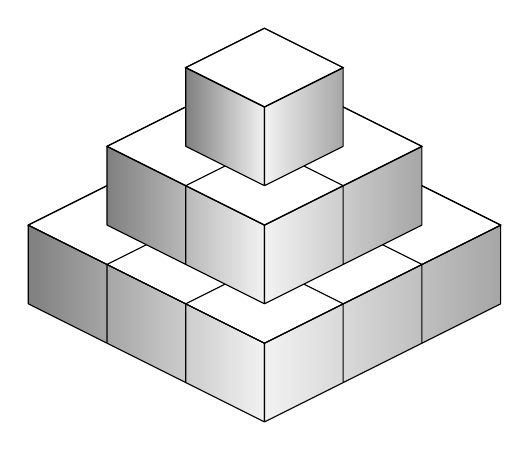
\begin{tikzpicture}
    \tikzset {
        cube layer/.pic = {
            \pgfmathsetmacro{\num}{#1}
            \shade[yslant=-0.5,right color=gray!10, left color=black!50] (0,0) rectangle +(\num,1);
            \draw [yslant=-0.5] (0,0) grid (\num,1);
            \shade[yslant=0.5,right color=gray!70,left color=gray!10] (\num,-\num) rectangle +(\num,1);
            \draw [yslant=0.5] (\num,-\num) grid (2*\num,1-\num);
            \draw [yslant=0.5,xslant=-1,fill=white] (1,1-\num) rectangle +(\num,\num);
            \draw [yslant=0.5,xslant=-1][fill=blue] (1,1-\num) grid (\num+1, 1);
        }
    }
    \path(0, 0) pic {cube layer=3};
    \path(1, 1) pic {cube layer=2};
    \path(2, 2) pic {cube layer=1};
\end{tikzpicture}
    \caption{}\label{fig:2-8}
\end{wrapfigure}

用这个公式可以计算如图 \ref{fig:2-8} 所示的一堆物品的总数。

\liti 用数学归纳法证明 $x^{2n} - y^{2n} \; (n \in N)$ 能被 $x + y$ 整除。

\zhengming (1) 当 $n = 1$ 时,$x^2 - y^2 = (x + y)(x - y)$ 能被 $x + y$ 整除。

(2) 假设当 $n = k\; (k \in N)$ 时,$x^{2k} - y^{2k}$ 能被 $x + y$ 整除,那么

\begin{align*}
      & x^{2(k+1)} - y^{2(k+1)} \\
    = & x^2 \cdot x^{2k} - y^2 \cdot y^{2k} \\
    = & x^2 \cdot x^{2k} - x^2 \cdot y^{2k} + x^2 \cdot y^{2k} - y^2 \cdot y^{2k} \\
    = & x^2(x^{2k} - y^{2k}) + y^{2k}(x^2 - y^2) \text{。}
\end{align*}

因为 $x^{2k} - y^{2k}$ 与 $x^2 - y^2$ 都能被 $x + y$ 整除,所以它们的和 $x^2(x^{2k} - y^{2k}) + y^{2k}(x^2 - y^2)$
也能被 $x + y$ 整除。这就是说,当 $n = k + 1$ 时,$x^{2(k+1)} - y^{2(k+1)}$ 能被 $x + y$ 整除。

根据 (1) 和 (2),可知命题对任何 $n \in N$ 都成立。


\liti 平面内有 $n$ 条直线,其中任何两条不平行,任何三条不过同一点,证明交点的个数 $f(n)$ 等于 $\dfrac{1}{2} n(n-1)$。

\zhengming (1) 当 $n = 2$ 时,两条直线的交点只有 $1$ 个,即 $f(2) = 1$。又当 $n = 2$ 时,
$$ \dfrac{1}{2} \times 2 \times (2 - 1) = 1 ,$$
因此命题成立。


\begin{wrapfigure}[10]{r}{7cm}
  \centering
  \begin{tikzpicture}
    \def \line(#1){a#1}
    \draw [name path=a1] (0, 0) -- (6.5,0);
    \draw [name path=a2] (0, -2.2) -- (6, 2.5);
    \draw [name path=a3] (1.3, -3.1) -- (3, 4);
    \draw [name path=a4] (5.6, -2.8) -- (2, 4);
    \draw [name path=a5] (6.7, -2.5) -- (0.2, 2.6);
    \foreach \x in {1,...,4} {
        \pgfmathtruncatemacro{\start}{\x+1}
        \foreach \y in {\start,...,5} {
            \filldraw [name intersections={of=\line(\x) and \line(\y), by=i}] (i) circle (0.1);
        }
    }

    \node at (1.7, 0.3) {$A_1$};
    \node at (2.5, 0.3) {$A_2$};
    \node at (4.3, 0.3) {$A_k$};
    \node at (6, 0.3) {$l$};
\end{tikzpicture}
  \caption{}\label{fig:2-9}
\end{wrapfigure}

(2) 假设 $n = k$ 时命题成立,就是说,平面内满足题设的任何 $k$ 条直线的交点的个数 $f(k)$ 等于 $\dfrac{1}{2} k(k - 1)$。
现在来考虑平面内有 $k + 1$ 条直线的情况。任取其中的 $1$ 条直线,记为 $l$ (图\ref{fig:2-9})。由上述归纳法的假设,
除 $l$ 以外的其他 $k$ 条直线的交点的个数 $f(k)$ 等于 $\dfrac{1}{2} k(k - 1)$ 。
另外,因为已知任何两条直线不平行,所以直线 $l$ 必与平面内其他 $k$ 条直线都相交;
又因为已知任何三条直线不过同一点,所以上面的 $k$ 个交点两两不相同,且与平面内其他的 $\dfrac{1}{2} k(k - 1)$ 个交点也两两不相同,
从而平面内交点的个数是

\begin{align*}
      & \dfrac{1}{2} k(k - 1) + k \\
    = & \dfrac{1}{2} k[(k - 1) + 2] \\
    = & \dfrac{1}{2} (k+1) [(k+1) - 1] \text{。}
\end{align*}

这就是说,当 $n=k+1$ 时, $k+1$ 条直线的交点个数 $f(k+1)$ 等于 $\dfrac{1}{2} (k+1) [(k+1) - 1]$ 。

根据 (1) 和 (2),可知命题对任何 $n \geqslant 2$ 且 $n \in N$ 都成立。


\liti 设 $\sin\dfrac{\alpha}{2} \neq 0$,用数学归纳法证明
$$ \sin \alpha + \sin 2\alpha + \sin 3\alpha + \cdots + \sin n\alpha = \dfrac{\sin \dfrac{n\alpha}{2} \sin \dfrac{(n+1)\alpha}{2}}{\sin \dfrac{\alpha}{2}} \text{。} $$

\zhengming (1) 当 $n = 1$ 时,左边是 $\sin\alpha$,右边是
$$ \dfrac{\sin \dfrac{\alpha}{2} \sin \alpha}{\sin \dfrac{\alpha}{2}} = \sin\alpha \text{,} $$
等式成立。

(2) 假设当 $n = k$ 时等式成立,就是
$$ \sin \alpha + \sin 2\alpha + \sin 3\alpha + \cdots + \sin k\alpha = \dfrac{\sin \dfrac{k\alpha}{2} \sin \dfrac{(k+1)\alpha}{2}}{\sin \dfrac{\alpha}{2}} \text{,} $$
那么,

\begin{align*}
      & \sin \alpha + \sin 2\alpha + \sin 3\alpha + \cdots + \sin k\alpha + \sin (k+1)\alpha \\
    = & \dfrac{\sin \dfrac{k\alpha}{2} \sin \dfrac{(k+1)\alpha}{2}}{\sin \dfrac{\alpha}{2}} + \sin (k+1)\alpha \\
    = & \dfrac{\sin \dfrac{k\alpha}{2} \sin \dfrac{(k+1)\alpha}{2} +  \sin \dfrac{\alpha}{2} \sin (k+1)\alpha}{\sin \dfrac{\alpha}{2}} \\
    = & \dfrac{\dfrac{1}{2} \left( \cos\dfrac{\alpha}{2} - \cos\dfrac{2k+1}{2}\alpha + \cos\dfrac{2k+1}{2}\alpha - \cos\dfrac{2k+3}{2}\alpha \right)}{\sin\dfrac{\alpha}{2}} \\
    = & \dfrac{\cos\dfrac{\alpha}{2} - \cos\dfrac{2k+3}{2}\alpha}{2\sin\dfrac{\alpha}{2}} \\
    = & \dfrac{\sin\dfrac{(k+1)\alpha}{2} \sin\dfrac{[(k+1)+1]\alpha}{2}}{\sin\dfrac{\alpha}{2}} \text{。}
\end{align*}

这就是说,当 $n = k + 1$ 时等式也成立。

根据 (1) 和 (2),可知等式对任何 $n \in N$ 都成立。


\lianxi

用数学归纳法证明:

\begin{xiaotis}

\xiaoti{$1 \cdot 2 + 2 \cdot 3 + 3 \cdot 4 + \cdots + n(n+1) = \dfrac{1}{3}n(n+1)(n+2)$。}

\xiaoti{$-1 + 3 - 5 + \cdots + (-1)^n (2n-1) = (-1)^n n$。}

\xiaoti{$x^n - y^n \; (n \in N)$ 能被 $x - y$ 整除。}

\xiaoti{凸 $n$ 边形的内角和 $f(n) = (n - 2) \pi \quad (n \geqslant 3)$。}

\end{xiaotis}


    \caption{}\label{fig:2-5}
\end{figure}

\jie 由题意可知,这个 V 形架上共放着 $120$ 层铅笔,且自下而上各层的铅笔数组成等差数列,记为 $\{a_n\}$,
其中 $a_1 = 1$,$a_{120} = 120$。根据等差数列 $\{a_n\}$ 前 $n$ 项和的公式,得
$$ S_{120} = \dfrac{120 \times (1 + 120)}{2} = 7260 \text{。}$$

答:V形架上共放着 $7260$ 支铅笔。

\liti 求集合 $M = \{ m \mid m = 7n ,\, n \in N \text{,且} m < 100 \}$ 的元素个数,并求这些元素的和。

\jie $\because \quad 7n < 100,$

$\therefore \quad \begin{aligned}[t]
     & n < \dfrac{100}{7} \\
     & n < 14\dfrac{2}{7} \text{。}
\end{aligned}$

由于满足上面不等式的自然数 $n$ 共有 $14$ 个,集合 $M$ 里的元素共有 $14$ 个。将它们从小到大列出,得
$$ 7,\; 7 \times 2,\; 7 \times 3,\; \cdots,\; 7 \times 14, $$
即
$$ 7,\; 14,\; 21,\; \cdots,\; 98 \text{。}$$
这个数列是等差数列,记为 $\{a_n\}$ ,其中 $a_1 = 7$, $a_{14} = 98$。因此,
$$ S_{14} = \dfrac{14 \times (7 + 98)}{2} = 735 \text{。} $$

答:集合 $M$ 共有 $14$ 个元素,它们的和等于 $735$ 。

例 5 表明,在小于 100 的正整数中共有 $14$ 个数是 $7$ 的倍数,它们的和是 $735$ 。

\liti 已经一个直角三角形的三条边的长成等差数列,求证它们的比是 $3:4:5$。

\zhengming 将成等差数列的三条边的长从小到大排列,它们可以表示为 $a - d$,$a$,$a + d$,
这里 $a - d > 0$, $d > 0$。由于它们是直角三角形的三条边的长,根据勾股定理,得到
$$ (a - d)^2 + a^2 = (a + d)^2 \text{。}$$

解得
$$ a = 4d \text{,}$$
从而这三条边的长是 $3d$,$4d$,$5d$。

因此,这三条边的长的比是 $3:4:5$。

\lianxi
\begin{xiaotis}
\setcounter{cntxiaoti}{0}

\xiaoti{根据下列各题中的条件,求相应的等差数列 $\{a_n\}$ 的 $S_n$:}
\begin{xiaoxiaotis}

    \xiaoxiaoti{$a_1 = 5$,$a_n = 95$,$n = 10$;}

    \xiaoxiaoti{$a_1 = 100$,$d = -2$,$n = 50$;}

    \xiaoxiaoti{$a_1 = \dfrac{2}{3}$,$a_n = -\dfrac{3}{2}$,$n = 14$;}

    \xiaoxiaoti{$a_1 = 14.5$,$d = 0.7$,$a_n = 32$。}

\end{xiaoxiaotis}

\xiaoti{}

\begin{xiaoxiaotis}

    \vspace{-1.6em} \begin{minipage}{0.9\textwidth}
    \xiaoxiaoti{求自然数列中前 $n$ 个数的和;}
    \end{minipage}

    \xiaoxiaoti{求自然数列中前 $n$ 个偶数的和。}

\end{xiaoxiaotis}
\end{xiaotis}






